\documentclass{article}
% For math environments
\usepackage{amsmath, amsfonts}
% For links
\usepackage[colorlinks=true,
    linkcolor = blue,
    urlcolor  = blue,
    citecolor = blue,
    anchorcolor = blue]{hyperref}
% Put space between paragraphs
\usepackage{parskip}
% For figures
\usepackage{tikz}
% Set the margins to not be ridiculous
\usepackage[margin=0.75in]{geometry}
% For multiple columns
\usepackage{multicol}
% For controlling enum/itemize spacing and indentation
\usepackage{enumitem}
% More math symbols
\usepackage{amssymb}
% To change enumerate labels

% For tikz plots
\usepackage{pgfplots}
% This isn't needed but avoids a compiler warning
\pgfplotsset{compat=1.16}

% Allow multi-line equations to be broken across pages
\allowdisplaybreaks

% Use @ as a letter
\makeatletter

% Scale down all tikz coordinates while maintaining font size
\tikzset{every picture/.style={scale=0.45, every picture/.style={}}}


% Macros
% Monospace code
\def\code#1{\texttt{#1}}

% Greek letters
\def\a{\alpha}
\def\b{\beta}
\def\g{\gamma}
\def\d{\delta}
\def\D{\Delta}

% Commands that make life easier
\newcommand\gath[1]{\begin{gather} #1 \end{gather}}
\newcommand\ali[1]{\begin{align} #1 \end{align}}
\newcommand\parens[1]{\left( #1 \right)}
\newcommand\squares[1]{\left[ #1 \right]}
\newcommand\braces[1]{\left\{ #1 \right\}}
\newcommand\angles[1]{\left\langle #1 \right\rangle}
\newcommand\deriv[2]{\frac{d #1}{d #2}}
\newcommand\abs[1]{\left| #1 \right|}
\newcommand\floor[1]{\left\lfloor #1 \right\rfloor}
\DeclareMathOperator{\lcm}{lcm}
\def\non{\nonumber \\}

% Multiline equation space
\def\mlesp{\hspace{1.2cm}}

% For grid diagrams
\newcommand\gridbox[3]{\draw (#1,#2) rectangle (#1+1,#2+1) node[pos=.5] {#3};}
\newcommand\gridboxh[3]{\draw[fill=red!20] (#1,#2) rectangle (#1+1,#2+1) node[pos=.5] {#3};}
\newcommand\gridboxb[3]{\draw[fill=black] (#1,#2) rectangle (#1+1,#2+1) node[pos=.5] {#3};}
\newcommand\gridsym[3]{\node at (#1+0.5,#2+0.5) {$#3$};}
\newcommand\gridblank[2]{\filldraw[draw=gray, color=gray] (#1,#2) rectangle (#1+1,#2+1);}
\newcommand\gridcirc[2]{\draw (#1 + 0.5,#2 + 0.5) circle (0.25);}
\newcommand\cwlab[3]{
  \def\dd{0.15}
  \draw (#1 + \dd - 0.03, #2 + 1 - \dd) node {\scriptsize #3};
}

\def\bbw{3.5}
\def\bbh{2}
\newcommand\bigbox[3]{\draw (#1*\bbw,#2*\bbh) rectangle (#1*\bbw+\bbw,#2*\bbh+\bbh) node[pos=.5] {#3};}
\newcommand\bbtextr[3]{\node[right] at (#1*\bbw,#2*\bbh+0.5*\bbh) {#3};}
\newcommand\bbtextb[3]{\node[align=center] at (#1*\bbw+0.5*\bbw,#2*\bbh+0.5*\bbh) {#3};}

% Box puzzle stock answer
\newcommand\boxans[1]{
  Logic was used to deduce the solution:

  #1

  This was verified using Python as well as shown to be unique with a brute force approach.
}

% Multiple numbers
\newcommand\mn[1]{$#1$'s}

% Commands for problems
\newcommand\problem[4]{
  \section*{#1}

  Question: #3
  
  Answer: #2
  
  Explanation: #4
}
\newcommand\aproblem[4]{\problem{Dec #1}{#2}{#3}{#4}}
\newcommand\cproblem[4]{\problem{Problem #1}{#2}{#3}{#4}}

\def\advent@xxiv@i{
  Eve writes down five different positive integers.
  The sum of her integers is $16$. What is the product of her integers?
}

\def\advent@xxiv@ii{
  $14$ is the smallest even number that cannot be obtained by rolling two $6$-sided dice and finding the product of the numbers rolled.

  What is the smallest even number that cannot be obtained by rolling one hundred $100$-sided dice and finding the product of the numbers rolled?
}

\def\advent@xxiv@iii{
  There are $5$ ways to write $5$ as the sum of positive odd numbers:
  \begin{itemize}
    \item $1 + 1 + 1 + 1 + 1$
    \item $1 + 1 + 3$
    \item $3 + 1 + 1$
    \item $1 + 3 + 1$
    \item $5$
  \end{itemize}

  How many ways are there to write $14$ as the sum of positive odd numbers?
}

\def\advent@xxiv@iv{
  The geometric mean of a set of $n$ numbers is computed by mulitplying all the numbers together, then taking the $n$th root.
  The factors of $9$ are $1$, $3$, and $9$.
  The geometric mean of these factors is
  \gath{
    \sqrt[3]{1 \times 3 \times 9} = \sqrt[3]{27} = 3
  }
  What is the smallest number where the geometric mean of its factors is $13$?
}

\def\advent@xxiv@v{
  The sum of $11$ consecutive integers is $2024$.
  What is the smallest of the $11$ integers?
}

\def\advent@xxiv@vi{Put the digits 1 to 9 (using each digit exactly once) in the boxes so that the sums are correct. The sums should be read left to right and top to bottom ignoring the usual order of operations. For example, 4+3×2 is 14, not 10. Today's number is the product of the numbers in the red boxes.
  The number $n$ has $55$ digits.
  All of its digits are $9$.
  What is the sum of the digits of $n^3$?
}

\def\advent@xxiv@vii{
  What is the obtuse angle in degrees between the minute and hour hands of a clock at 08:22?
}

\def\advent@xxiv@viii{
  It is possible to arrange $4$ points on a plane and draw non-intersecting lines between them to form $3$ non-overlapping triangles:

  \begin{center}
    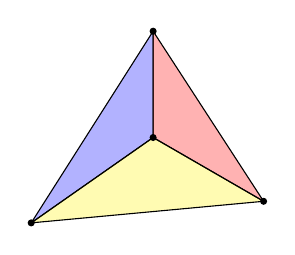
\begin{tikzpicture}
      \def\ds{3}
      \def\pa{(0: 0)}
      \def\pb{(90: \ds)}
      \def\pc{(215: 1.4*\ds)}
      \def\pd{(-30: 1.2*\ds)}

      \def\bcr{3}
      \def\scr{0.55*\bcr}
      \def\sca{34}
      \def\mcr{0.7*\bcr}
      \def\mca{142}
      \def\pr{0.1}

      % Triangles
      \draw[fill=blue,fill opacity=0.3] \pa -- \pb -- \pc -- cycle;
      \draw[fill=red,fill opacity=0.3] \pa -- \pb -- \pd -- cycle;
      \draw[fill=yellow,fill opacity=0.3] \pa -- \pd -- \pc -- cycle;

      % Points
      \fill \pa circle (\pr);
      \fill \pb circle (\pr);
      \fill \pc circle (\pr);
      \fill \pd circle (\pr);
    \end{tikzpicture}
  \end{center}

  It is not possible to make more than $3$ triangles with $4$ points.

  What is the maximum number of non-overlapping triangles that can be made by arranging $290$ points on a plane and drawing non-intersecting lines between them?
}

\def\advent@xxiv@ix{
  Put the digits $1$ to $9$ (using each digit exactly once) in the boxes so that the sums are correct.
  The sums should be read left to right and top to bottom ignoring the usual order of operations.
  For example, $4 + 3 \times 2$ is $14$, not $10$.
  Today's number is the product of the numbers in the red boxes.

  \grid@advent@xxiv@ix{}{}{}{}{}{}{}{}{}
}

\def\advent@xxiv@x{
  A number is a palindrome if it's the same when its digits are written in reverse order.

  What is the sum of all the numbers between $10$ and $100$ that are palindromes?
}

\def\advent@xxiv@xi{
  There are $6$ sets of integers between $1$ and $5$ (inclusive) that contain an odd number of numbers whose median value is $3$:

  \begin{itemize}
    \item $\braces{3}$
    \item $\braces{1,3,4}$
    \item $\braces{2,3,4}$
    \item $\braces{1,3,5}$
    \item $\braces{2,3,5}$
    \item $\braces{1,2,3,4,5}$
  \end{itemize}

  How many sets of integers between $1$ and $11$ (inclusive) are there that contain an odd number of numbers whose median value is $5$?
}

\def\advent@xxiv@xii{
  Holly picks a three-digit number.
  She then makes a two-digit number by removing one of the digits.
  The sum of her two numbers is $309$.
  What was Holly's original three-digit number?
}

\def\advent@xxiv@xiii{
  Today's number is given in this crossnumber.
  No number in the completed grid starts with $0$.

  \begin{multicols}{2}
    \crossnumstd{}{}{}{}{}{}{}{}{}

    \vfill\null
    \columnbreak

    \begin{center}
      \textbf{Across}

      \begin{tabular}{clc}
        \textbf{1} & Today's number.  & (\textbf{3}) \\
        \textbf{4} & Two times 5A.    & (\textbf{3}) \\
        \textbf{5} & A multiple of 1. & (\textbf{3})
      \end{tabular}

      \textbf{Down}

      \begin{tabular}{clc}
        \textbf{1} & Sum of digits is 15. & (\textbf{3}) \\
        \textbf{2} & Sum of digits is 19. & (\textbf{3}) \\
        \textbf{3} & Three times 5A.      & (\textbf{3})
      \end{tabular}
    \end{center}
  \end{multicols}
}

\def\advent@xxiv@xiv{
  $15^3$ is $3375$.
  The last $3$ digits of $15^3$ are $375$.

  What are the last $3$ digits of $15^{1234567890}$?
}

\def\advent@xxiv@xv{
  The number $2268$ is equal to the product of a square number (whose last digit is not $0$) and the same square number with its digits reversed: $36 \times 63$.

  What is the smallest three-digit number that is equal to the product of a square number (whose last digit is not $0$) and the same square number with its digits reversed?
}

\def\advent@xxiv@xvi{
  Put the digits $1$ to $9$ (using each digit exactly once) in the boxes so that the sums are correct.
  The sums should be read left to right and top to bottom ignoring the usual order of operations.
  For example, $4 + 3 \times 2$ is $14$, not $10$.
  Today's number is the product of the numbers in the red boxes.

  \grid@advent@xxiv@xvi{}{}{}{}{}{}{}{}{}
}

\def\advent@xxiv@xvii{
  The number $40$ has $8$ factors: $1$, $2$, $4$, $5$, $8$, $10$, $20$, and $40$.

  How many factors does the number $2^{26} \times 5 \times 7^5 \times 11^2$ have?
}

\def\advent@xxiv@xviii{
  TODO
}

\def\card@xxiv@i{
  What is the largest number you can make by using the digits $1$ to $4$ to make two $2$-digit numbers, then mutiplying the two numbers together?
}

\def\card@xxiv@ii{
  What is the largest number you can make by using the digits $0$ to $9$ to make a $2$-digit number and an $8$-digit number, then mutiplying the two numbers together?
}

\def\card@xxiv@iii{
  The expansion of $(2x+3)^2$ is $4x^2 + 12x + 9$.
  The sum of the coefficients of $4x^2 + 12x + 9$ is $25$.
  What is the sum of the coefficients of the expansion of $(30x + 5)^2$?
}

\def\card@xxiv@iv{
  What is the sum of the coefficients of the expansion of $(2x+1)^{11}$?
}

\def\card@xxiv@v{
  What is the geometric mean of all the factors of $41306329$?
}

\def\card@xxiv@vi{
  What is the largest number for which the geometric mean of all its factors is $92$?
}

\def\card@xxiv@vii{
  What is the sum of all the factors of $7^4$?
}

\def\card@xxiv@viii{
  How many numbers between $1$ and $28988500000$ have an odd number of factors?
}

\def\card@xxiv@ix{
  Eve found the total of the $365$ consecutive integers starting at $500$ and the total of the next $365$ consecutive integers, then subtracted the smaller total from the larger total.
  What was her result?
}

\def\card@xxiv@x{
  Eve found the total of the $n$ consecutive integers starting at a number and the total of the next $n$ consecutive integers, then subtracted the smaller total from the larger total.
  Her result was $22344529$.
  What is the largest possible value of $n$ that she could have used?
}

\input{boxes}

\begin{document}

\title{MS Scroggs Advent Calendar 2023 Answers}
\author{Dan Whitman}
\date{}

\maketitle

Magic Link: \href{http://mscroggs.co.uk/adventcode/yglswiTw}{http://mscroggs.co.uk/adventcode/yglswiTw}

\aproblem{1}{180}{\advent@xxiii@i}{
  A regular $n$-gon has interior angles that are each
  \gath{
    \theta = \frac{180(n - 2)}{n}
  }
  in degrees.
  Using basic algebra, solving this for $n$ results in
  \gath{
    n = \frac{360}{180 - \theta}
  }
  Therefore, plugging in $\theta = 178$ gives our answer $n = 180$.
}

\aproblem{2}{681}{\advent@xxiii@ii}{
  Clearly, the sum of the first $n$ even numbers and half of the next even number is
  \ali{
    s_n &= \sum_{i=1}^n 2i + \frac{2(n+1)}{2} = 2 \sum_{i=1}^n i + (n+1) = 2\frac{n(n+1)}{2} + (n+1) \non
    &= n(n+1) = (n+1) = (n+1)^2.
  }
  Solving this for $n$ clearly results in
  \gath{
    n = \sqrt{s_n} - 1.
  }
  Hence, the $n$ we seek is $n = \sqrt{465124} - 1 = 682 - 1 = 681$.
  This answer was verified with a Python program that calculates the actual sum $s_{681}$, showing that this is indeed $465124$.
}

\aproblem{3}{195}{\advent@xxiii@iii}{
  Let $n$ be this smallest multiple of $15$ whose digits add up to $15$.
  First, we note that clearly the digits of $555$ add to $15$, and that $555 = 37 \times 15$, and so is also a multiple of $15$.
  Therefore, it has to be that $n \leq 555$.

  Now, any multiple of $15$ must end in either the digits $0$ or $5$.
  Suppose that the last digit is $0$ so that $n$ has the form $n = d_2 d_10$, and thus $d_2 + d_1 = 15$.
  There are only two sets of digits such that this is the case, namely $6 + 9 = 9 + 6 = 15$ and $7 + 8 = 8 + 7 = 15$.
  This is because $d_2 \leq 5$ would require that $d_1 > 9$ and vice versa.
  Therefore, it has to be that $d_2 \in \braces{6, 7, 8, 9}$, which would mean that $n = d_2 d_1 0 > 555$.
  Hence, it must be that the last digit is a $5$.

  Thus, $n$ has the form $n = d_2 d_1 5$.
  If it were the case that $d_2 = 0$ so that $n$ was a two-digit number, it would have to be that $0 + d_1 + 5 = 15$ so that $d_1 = 10$, which is clearly out of the range of valid digits.
  Therefore, $0 < d_2 \leq 5$.
  What about if $d_2 = 1$?
  Well, in this case, we'd have $1 + d_2 + 5 = 15$ so that $d_2 = 9$.
  Hence, the digits of $n = 195$ sum to $15$.
  Since also $195 = 13 \times 15$, this is in fact our answer since there can be no smaller number that meets the established criteria!

  This answer was also verified using a brute force Python program.
}

\aproblem{4}{246}{\advent@xxiii@iv}{
  Let us generalize this a bit and ask, for any positive integer $a$, what is the largest value of $n$ for which $f(n) = (n! - a)/(n - a)$ is an integer?

  First, for $n = 2a$ we have
  \gath{
    f(n) = f(2a) = \frac{(2a)! - a}{2a - a} = \frac{2a(2a-1)! - a}{a} = 2(2a-1)! - 1,
  }
  which is clearly an integer. We aim to prove that, in fact, $n = 2a$ is the \emph{largest} $n$ for which $f(n)$ is an integer!

  To this end, first note that $f(n)$ being an integer means that $n! - a$ is divisible by $n - a$, which is equivalent to saying that
  \gath{
    n! - a \equiv 0 \pmod{n-a}. \label{eqn:04:fcond}
  }
  Now suppose that $n > 2a$ so that
  \gath{
    a > 0 \non
    n > 2a > a \non
    n - a > a > 0.
  }
  We also clearly have
  \gath{
    n > n - a
  }
  since $a > 0$.
  Therefore, clearly
  \gath{
    n! = (n-a)k,
  }
  where $k$ is an integer.
  Hence, $n!$ is a multiple of $n-a$ so that
  \gath{
    n! \equiv 0 \pmod{n-a}.
  }
  From this it follows that
  \gath{
    n! - a \equiv -a \pmod{n-a},
  }
  and, since $0 < a < n-a$, this means that \eqref{eqn:04:fcond} cannot be true so that $f(n)$ cannot be an integer!

  In our case, we have $a = 123$ so that our answer is $n = 2 \cdot 123 = 246$.
  This answer was also verified using a brute force Python program.
}

\aproblem{5}{378}{\advent@xxiii@v}{
  \boxans{\gridsol@advent@xxiii@v}
}

\aproblem{6}{233}{\advent@xxiii@vi}{
  Consider the general problem of the number of ways to tile a $k \times 2$ rectangle with $2 \times 1$ pieces.
  Clearly one way, for all $k \geq 1$, is for all the $2 \times 1$ pieces to be oriented vertically.
  As any adjacent pair of $2 \times 1$ pieces forms a square, the pair can be oriented either with the pieces vertically or horizontally.
  So the problem is equivalent to considering $k$ items lined up in a row and counting the number of ways that zero or more adjacent pairs can be chosen.
  A chosen pair corresponds to the pair being oriented horizontally instead of the default vertical orientation.
  Obviously a single item cannot be shared between two distinct adjacent pairs, and so can only be chosen at most once.

  So, using the ways to tile a $4 \times 2$ rectangle above as an example, if we label each of the vertical $2 \times 1$ pieces from left to right as $1$, $2$, $3$, and $4$, then each of the five arrangements corresponds to the following chosen adjacent pairs:
  % Ugh, evidently there's no way to just easily vertically center the text in a way that works with teh graphics!
  \begin{center}
    \begin{tabular}{cm{4cm}}
      Arrangement \vspace{6pt} & Chosen adjacent pairs    \\
      \begin{tikzpicture}[scale=\crscale]
        \crfour@i{0}{0}
      \end{tikzpicture}
                               & $\varnothing$            \\
      \begin{tikzpicture}[scale=\crscale]
        \crfour@ii{0}{0}
      \end{tikzpicture}
                               & $\braces{\braces{3, 4}}$ \\
    \end{tabular}
  \end{center}
}

\end{document}
